\documentclass[letterpaper,12pt]{article}

\usepackage[margin=1in]{geometry}
\usepackage{amsthm}
\usepackage{parskip}
\usepackage{tasks}
\usepackage{fancyhdr}
\usepackage{titling}

% Typography and font packages.
\usepackage{lmodern}
\usepackage{microtype}

% Math packages.
\usepackage{amsmath}
\usepackage{amssymb}
\usepackage{mathtools}
\usepackage{commath}
\usepackage{siunitx}

\frenchspacing

% Macros for math
\newcommand{\such}{\mid}
\newcommand{\real}{\mathbb{R}}
\newcommand{\integer}{\mathbb{Z}}
\DeclarePairedDelimiter{\ceil}{\lceil}{\rceil}
\DeclarePairedDelimiter{\floor}{\lfloor}{\rfloor}

% Unit setup
\NewDocumentCommand{\varSI}{}{\SI[number-math-rm=\mathnormal,parse-numbers=false]} % Use variables as the value of units.


\newcommand{\solutionspace}[1]{\vspace{#1}~\newline}

% Redefine the page style.
\pagestyle{fancy}
\renewcommand{\headrulewidth}{1pt}
\renewcommand{\footrulewidth}{0.4pt}
\lhead{\theauthor}
\chead{\LARGE\thetitle}
\rhead{\thedate}
\cfoot{Page \thepage}
\lfoot{\texttt{mackenziemathclub.github.io}}


\usepackage{cleveref}
\usepackage{tikz}
\usepackage{tkz-euclide}
\usetikzlibrary{angles,quotes}
\usetkzobj{all}

\title{Euclid Preparation 3}
\author{Mackenzie Math Club}
\date{March 19, 2017}

\rfoot{\parbox[t]{0.35\textwidth}{\copyright{} Caroline Liu, Vincent Macri, and Samantha Unger, 2018}} 

\theoremstyle{definition}
\newtheorem{theorem}{Theorem}
\newtheorem{extension}{Extension}[theorem]
\newtheorem*{properties}{Properties}

\newenvironment{TheoremSide}[1]{\begin{minipage}{0.7\textwidth}\begin{theorem}[#1]~\\}{\end{theorem}\end{minipage}}
\newenvironment{ExtensionSide}[1]{\begin{minipage}{0.7\textwidth}\begin{extension}[#1]~\\}{\end{extension}\end{minipage}}
\newenvironment{DiagramSide}{\begin{minipage}[c][4cm]{0.3\textwidth}\centering}{\end{minipage}}
\newenvironment{PropertiesSide}[1]{\begin{minipage}{0.7\textwidth}\begin{properties}[#1]~\\}{\end{properties}\end{minipage}}

\begin{document}
	\begin{TheoremSide}{``Star Trek'' theorem}
			\label{starTrek}
			The central angle \emph{subtended} by any arc is twice any of the inscribed angles on that arc.
			\[\angle AOB = 2 \angle ACB\]
	\end{TheoremSide}
	\begin{DiagramSide}
		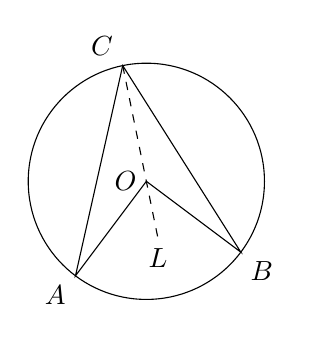
\begin{tikzpicture}[scale=0.3]
			\coordinate [label=left:$O$](O) at (0,0);
			\coordinate [label=below left:$A$](A) at (-3,-4);
			\coordinate [label=below right:$B$](B) at (4,-3);
			\coordinate [label=above left:$C$](C) at (-1,4.89897948557);
			\coordinate [label=below:$L$](L) at (0.5,-2.44948974278);

			\draw (O) circle (5);
			\draw (A) -- (O) -- (B) -- (C) -- cycle;
			\draw [dashed] (C) -- (L);
		\end{tikzpicture}
	\end{DiagramSide}
	\hrule
	\begin{ExtensionSide}{Diameters and right angles}
		If the chord $AB$ is a diameter then $\angle ACB = \SI{90}{\degree}$.
	\end{ExtensionSide}
	\begin{DiagramSide}
		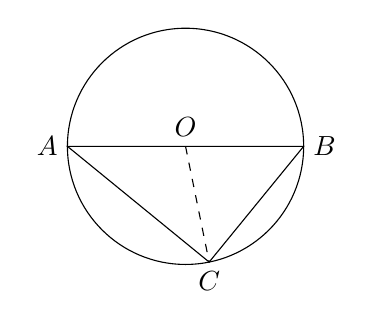
\begin{tikzpicture}[scale=0.3]
			\coordinate [label=above:$O$](O) at (0,0);
			\coordinate [label=left:$A$](A) at (-5,0);
			\coordinate [label=right:$B$](B) at (5,0);
			\coordinate [label=below:$C$](C) at (1,-4.89897948557);

			\draw (O) circle (5);
			\draw (A) -- (O) -- (B) -- (C) -- cycle;
			\draw [dashed] (O) -- (C);
		\end{tikzpicture}
	\end{DiagramSide}
	\hrule
	\begin{ExtensionSide}{On the major arc}
		\Cref{starTrek} is still true if $\angle AOB > \SI{180}{\degree}$.

		\[\angle AOB = 2\angle ACB\]
	\end{ExtensionSide}
	\begin{DiagramSide}
		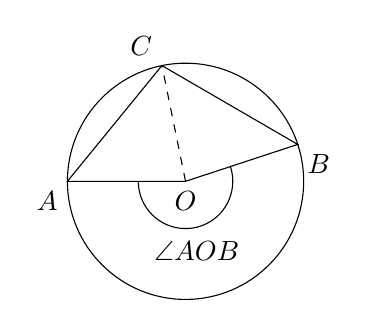
\begin{tikzpicture}[scale=0.3]
			\coordinate [label=below:$O$](O) at (0,0);
			\coordinate [label=below left:$A$](A) at (-5,0);
			\coordinate [label=below right:$B$](B) at (4.75,1.5612494996);
			\coordinate [label=above left:$C$](C) at (-1,4.89897948557);

			\draw (O) circle (5);
			\draw (A) -- (O) -- (B) -- (C) -- cycle;
			\draw [dashed] (O) -- (C);

			\pic [draw, "$\angle AOB$", angle eccentricity=1.5, angle radius=6mm] {angle = A--O--B};
		\end{tikzpicture}
	\end{DiagramSide}
	\hrule
	\begin{ExtensionSide}{Intersecting}
		\Cref{starTrek} is still true if the point $C$ is chosen so that $AB$ and $OB$ intersect.
		\[\angle AOC = 2 \angle ACB\]
	\end{ExtensionSide}
	\begin{DiagramSide}
		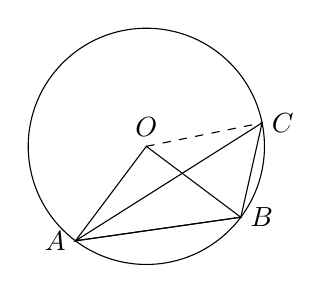
\begin{tikzpicture}[scale=0.3]
			\coordinate [label=above:$O$](O) at (0,0);
			\coordinate [label=left:$A$](A) at (-3,-4);
			\coordinate [label=right:$B$](B) at (4,-3);
			\coordinate [label=right:$C$](C) at (4.9,0.994987437107);

			\draw (O) circle (5);
			\draw (A) -- (B) -- (C) -- cycle;
			\draw (A) -- (B) -- (O) -- cycle;
			\draw [dashed] (O) -- (C);
		\end{tikzpicture}
	\end{DiagramSide}
	\hrule
	\begin{ExtensionSide}{Cyclic quadrilaterals}
		If $C_1$ and $C_2$ are two points on the circle, one on the minor arc $AB$ and the other on the major arc, then $\angle AC_1B + \angle AC_2B = \SI{180}{\degree}$.

		This is equivalent to proving that the opposite angles of a cyclic quadrilateral are supplementary.
	\end{ExtensionSide}
	\begin{DiagramSide}
		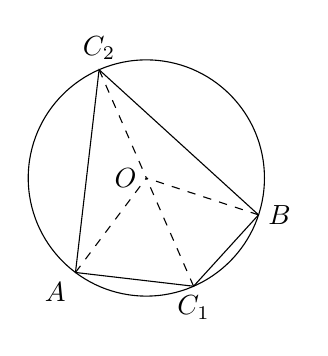
\begin{tikzpicture}[scale=0.3]
			\coordinate [label=left:$O$](O) at (0,0);
			\coordinate [label=below left:$A$](A) at (-3,-4);
			\coordinate [label=right:$B$](B) at (4.75,-1.5612494996);
			\coordinate [label=below:$C_1$](C1) at (2,-4.58257569496);
			\coordinate [label=above:$C_2$](C2) at (-2,4.58257569496);

			\draw (O) circle (5);
			\draw (A) -- (C1) -- (B) -- (C2) -- cycle;
			\draw [dashed] (A) -- (O);
			\draw [dashed] (B) -- (O);
			\draw [dashed] (C1) -- (O);
			\draw [dashed] (C2) -- (O);
		\end{tikzpicture}
	\end{DiagramSide}
	\begin{ExtensionSide}{Angles subtended by the same arc}
		If $C_1$ and $C_2$ are two different choices for the position of the point $C$ along the same arc $AB$ then $\angle AC_1B = \angle AC_2B$.

		This is equivalent to saying that angles subtended by the same arc are equal.
	\end{ExtensionSide}
	\begin{DiagramSide}
		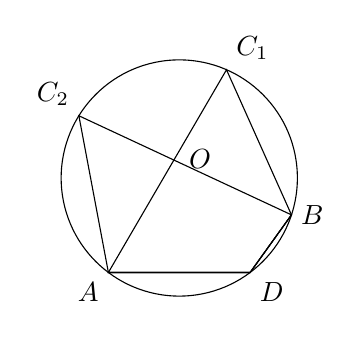
\begin{tikzpicture}[scale=0.3]
			\coordinate [label=above right:$O$](O) at (0,0);
			\coordinate [label=below left:$A$](A) at (-3,-4);
			\coordinate [label=right:$B$](B) at (4.75,-1.5612494996);
			\coordinate [label=above right:$C_1$](C1) at (2,4.58257569496);
			\coordinate [label=above left:$C_2$](C2) at (-4.25,2.63391343821);
			\coordinate [label=below right:$D$](D) at (3,-4);

			\draw (O) circle (5);
			\draw (A) -- (C2) -- (B) -- (D) -- cycle;
			\draw (A) -- (C1) -- (B) -- (D) -- cycle;
			\draw (A) -- (D) -- (B);
		\end{tikzpicture}
	\end{DiagramSide}
	\hrule
	\begin{TheoremSide}{Crossed chord theorem}
		If two chords $AB$ and $CD$ of a circle intersect at point $P$, then $(PA)(PB) = (PC)(PD)$.
	\end{TheoremSide}
	\begin{DiagramSide}
		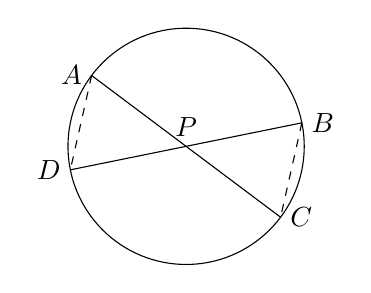
\begin{tikzpicture}[scale=0.3]
			\coordinate [label=above:$P$](P) at (0,0);
			\coordinate [label=left:$A$](A) at (-4,3);
			\coordinate [label=right:$B$](B) at (4.9,0.994987437107);
			\coordinate [label=right:$C$](C) at (4,-3);
			\coordinate [label=left:$D$](D) at (-4.9,-0.994987437107);

			\draw (P) circle (5);
			\draw (A) -- (P) -- (B);
			\draw (D) -- (P) -- (C);
			\draw [dashed] (B) -- (C);
			\draw [dashed] (A) -- (D);
		\end{tikzpicture}
	\end{DiagramSide}
	\hrule
	\begin{ExtensionSide}{Secant and tangents}
		If $PAB$ and $PCD$ are two secants of the same circle and they intersect at a point $P$ outside the circle then:
		\[(PA)(PB) = (PC)(PD)\]

		Additionally, if $PT$ is a tangent to the circle, then:
		\[(PA)(PB) = (PT)^2\]
	\end{ExtensionSide}
	\begin{DiagramSide}
		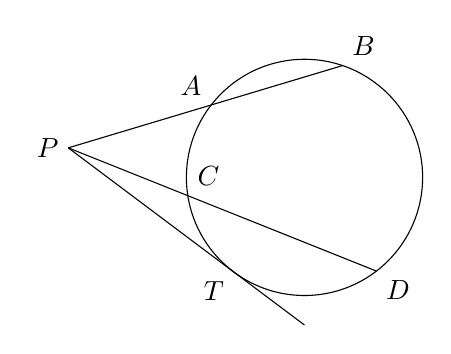
\begin{tikzpicture}[scale=0.3]
			\coordinate (O) at (0,0);
			\coordinate [label=left:$P$](P) at (-10,1.25);
			\coordinate [label=below left:$T$](T) at (-3,-4);
			\coordinate (E) at (0,-6.25);

			\coordinate [label=above left:$A$](A) at (-3.951,3.065);
			\coordinate [label=above right:$B$](B) at (1.611,4.733);
			\coordinate [label=above right:$C$](C) at (-4.94,-0.774);
			\coordinate [label=below right:$D$](D) at (3.043,-3.967);

			\draw (O) circle (5);
			\draw (P) -- (A) -- (B);
			\draw (P) -- (C) -- (D);
			\draw (P) -- (T) -- (E);
		\end{tikzpicture}
	\end{DiagramSide}
	\hrule
	\begin{PropertiesSide}{Properties of two tangents}
		If $P$ is a point outside of a circle and $PT$ and $PS$ are two tangents to the circle, then the following are true:
		\begin{enumerate}
			\item A tangent at a point on a circle is perpendicular to the radius draw to the point.
			\item $PS = PT$: tangents to a circle from an external point are equal.
			\item $OP$ bisects the angle between the tangents.
		\end{enumerate}
	\end{PropertiesSide}
	\begin{DiagramSide}
		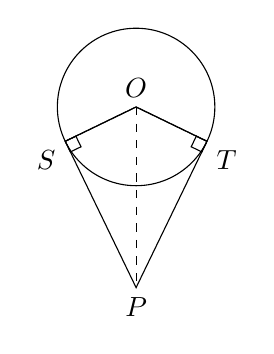
\begin{tikzpicture}[scale=0.2]
				\coordinate [label=above:$O$](O) at (0,0);
				\coordinate [label=below:$P$](P) at (0,-11.4707866935);
				\coordinate [label=below left:$S$](S) at (-4.5,-2.17944947177);
				\coordinate [label=below right:$T$](T) at (4.5,-2.17944947177);

				\draw (O) circle (5);
				\draw (P) -- (S) -- (O) -- (T) -- cycle;

				\tkzMarkRightAngle[size=0.75](P,S,O);
				\tkzMarkRightAngle[size=0.75](P,T,O);
				\draw [dashed] (O) -- (P);
				\draw (S) -- (O) -- (T);
		\end{tikzpicture}
	\end{DiagramSide}
	\hrule
	\begin{TheoremSide}{Tangent chord theorem}
		Given that $TA$ is any chord of a circle and $PT$ is a tangent to the circle at $T$.
		If $C$ is a point on the circle chosen to be on the side of the chord opposite to the tangent then $\angle TCA = \angle PTA$.
	\end{TheoremSide}
	\begin{DiagramSide}
		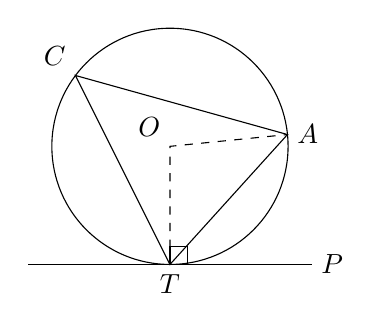
\begin{tikzpicture}[scale=0.3]
			\coordinate [label=above left:$O$](O) at (0,0);
			\coordinate [label=right:$P$](P) at (6,-5);
			\coordinate [label=below:$T$](T) at (0,-5);
			\coordinate (E) at (-6,-5);
			\coordinate [label=right:$A$](A) at (4.975, 0.499374608886);
			\coordinate [label=above left:$C$](C) at (-4, 3);

			\draw (O) circle (5);
			\draw (P) -- (T) -- (E);
			\draw (A) -- (C) -- (T) -- cycle;

			\draw [dashed] (T) -- (O) -- (A);

			\tkzMarkRightAngle[size=0.75](O,T,P);
		\end{tikzpicture}
	\end{DiagramSide}
\end{document}
